\documentclass[tikz]{standalone}
\usepackage{tikz}
\usetikzlibrary{positioning, arrows.meta} 

\begin{center}
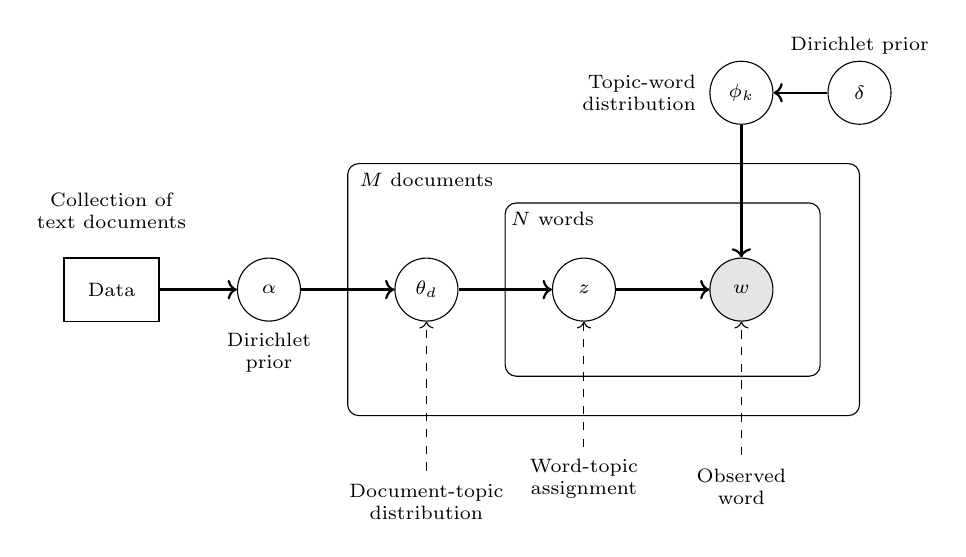
\begin{tikzpicture}[
  node distance=1.2cm and 1.6cm,
  every node/.style={font=\scriptsize},
  round/.style={circle, draw, minimum size=0.8cm},
  plate/.style={draw, rectangle, rounded corners, inner sep=10pt}
]

% Dataset stack
\node[draw, minimum width=1.2cm, minimum height=0.8cm] (dataset) at (-6,0) {Data};
\foreach \i in {1,...,6} {
  \draw[shift={(-0.1*\i, 0.1*\i)}] (dataset.north west) rectangle (dataset.south east);
}

% Alpha to theta
\node[round] (alpha) at (-4,0) {$\alpha$};
\node[round] (theta) at (-2,0) {$\theta_d$};
\draw[->, thick] (dataset.east) -- (alpha);
\draw[->, thick] (alpha) -- (theta);

% Document plate
\node[plate, minimum width=6.5cm, minimum height=3.2cm] (docplate) at (0.25,0) {};

% Inner plate for words
\node[plate, minimum width=4cm, minimum height=2.2cm] at (1,0) {};

% z and w
\node[round] (z) at (0,0) {$z$};
\node[round, fill=gray!20] (w) at (2,0) {$w$};
\draw[->, thick] (theta) -- (z);
\draw[->, thick] (z) -- (w);

% phi to w
\node[round] (delta) at (3.5,2.5) {$\delta$};
\node[round] (phi) at (2,2.5) {$\phi_k$};
\draw[->, thick] (phi) -- (w);
\draw[->, thick] (delta) -- (phi);

% External labels with arrows
\node[align=center, font=\scriptsize] at (-6,1) {Collection of\\text documents};

\node[align=center, font=\scriptsize] at (-4,-0.8) {Dirichlet\\prior};

\node[align=center, font=\scriptsize] at (-2,-2.7) {Document-topic\\distribution};
\draw[->, dashed] (-2,-2.3) -- (theta.south);

\node[align=center, font=\scriptsize] at (0,-2.4) {Word-topic\\assignment};
\draw[->, dashed] (0,-2) -- (z.south);

\node[align=center, font=\scriptsize] at (2,-2.5) {Observed\\word};
\draw[->, dashed] (2,-2.1) -- (w.south);

\node[align=right, font=\scriptsize] at (0.7,2.5) {Topic-word\\distribution};

\node[align=center, font=\scriptsize] at (3.5,3.1) {Dirichlet prior};

% Plate labels
\node[align=left, font=\scriptsize] at (-0.4,0.9) {$N$ words};
\node[align=left, font=\scriptsize] at (-2,1.4) {$M$ documents};

\end{tikzpicture}
\end{center}
\end{document}
